\clearpage
\section{Validation}\label{sec:validation}
% some end thing about our performance after it hits challenge requirements
\vspace{-0.2cm} After 10 weeks of workshops and hard fought open lab workshops, on 21 October 2019, 15:15 the designed algorithms and FSM was put to the final test on a novel obstacle course. The obstacle course was approximately 3m by 5m with a total of seven different obstacles in the area, which funnelled to an uphill ramp, plateau and downhill ramp. The starting and end lines were marked out by tape.

\subsection{Endgame - The Final Run}\label{sec:finalrun}
\vspace{-0.2cm} The Kobuki did not succeed in the final obstacle course. We chose to end the Kobuki around 90 seconds into the run as the robot seemed to have lost it's ground orientation so continuing would not have led it through the course. Because the Kobuki did not reach the hill climb section of the course, this part was not tested. Had we been given the chance to run the robot from the last obstacle and demonstrate hill climb, we are confident that the hill climb algorithm is robust through tests on a similar ramp and will be able to demonstrate project requirements to climb the hill, reorient, detect cliffs and stop after descent within 40cm. The relevant testing and design choices are covered in Section \ref{sec:hill_alg} and Section \ref{sec:hill_test}. Figure \ref{fig:KobukiFinalPath} shows the Kobuki's path through the given obstacle course, note the diagram is not to scale. Red shows the initial path with the centre bumper on default turning left and orange shows the path carried out after encountering the wall as an obstacle during obstacle avoidance. The start and finish lines are in yellow.
\begin{figure}[H]
    \centering
    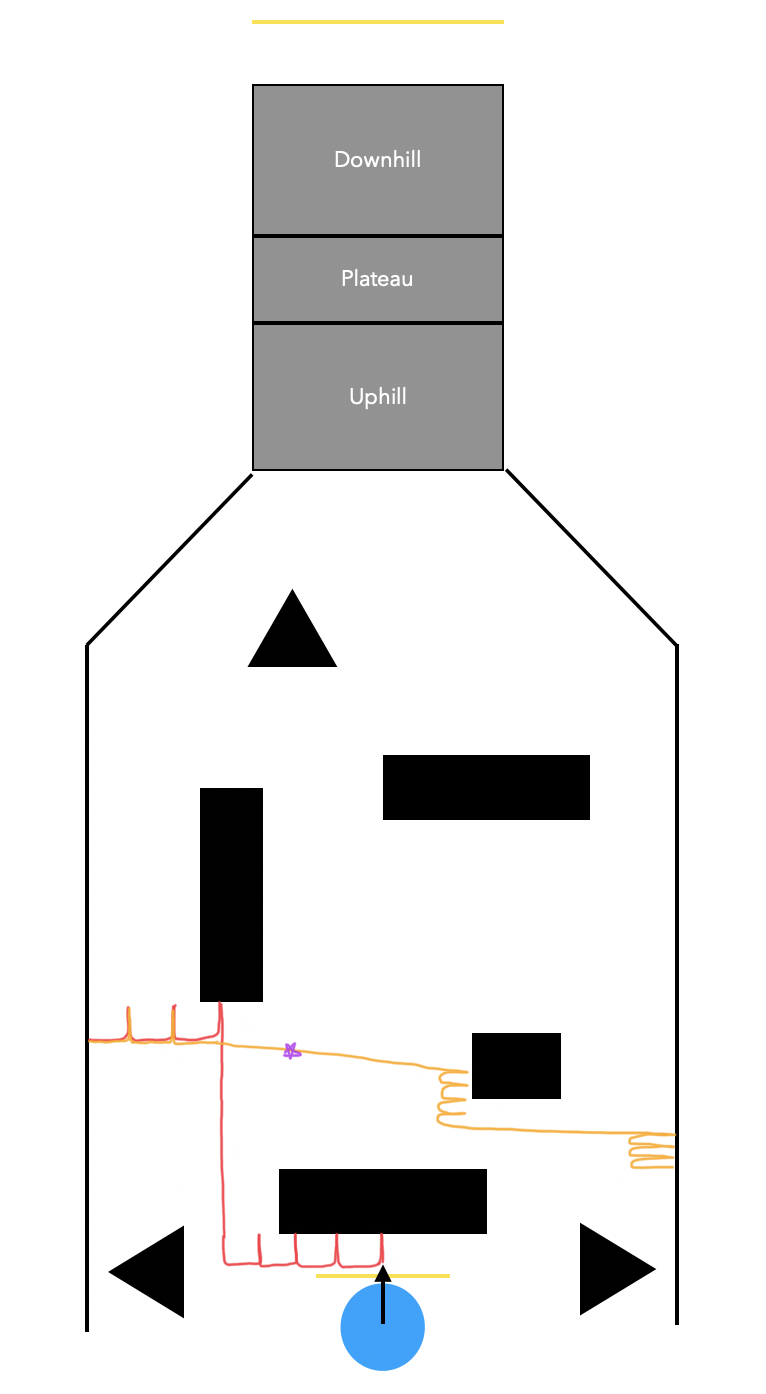
\includegraphics[width=8cm]{Images/KobukiFinalPath.png}
    \caption{Final obstacle course showing the Kobuki path}
    \label{fig:KobukiFinalPath}
\end{figure}

Analysing the outcome (through repeatedly watching the video taken of the final run), there was a clear point where the behaviour of the Kobuki became unexpected and this is labelled by a purple star in Figure \ref{fig:KobukiFinalPath}. The obstacle avoidance worked as expected, including the corner state sequence via \textit{ReverseCorner} to turn back and exhibit the centre bumper now turning right when triggered. The purple point what where the Kobuki should have reoriented towards the slope in the original ground orientation. However, there was a little hiccup seen in the videos, where the Kobuki was seen to rise. A theory is that it may have triggered the hill climb state \textit{Ascending} even though it's unlikely that the slant was more than $11.5^\circ$. But, indicators that support this theory, include the motion seeming to be more of an arc, which coincides with the reorientation feedback loop we have implemented, and the ground orientation was completely lost. Furthermore, during hill climb, obstacle detection was shown to be possible from our previous testing but after encountering obstacles after the purple star moment, the Kobuki seemed to continuously head bump. A theory to explain this could be that two sensors, both right and centre were bumped at the same time leading to the confusion for which side to turn, where the \texttt{centreTurne = true} leading to turn right and \textit{TurnAway} for the right bumper leads to turn left. However, there was no tangible evidence or state outputs from the final run to analyse the behaviour and conclude with confidence (laptops were not allowed).

%Our Kobuki did not manage to pass the obstacle course. Our Kobuki was doing fine at the beginning, successfully avoid some obstacles. However, when Kobuki is at 'DriveAvoid' state to avoid a obstacle, our Kobuki keep driving straight even the parallel distance has reached. Then our kuboki can not perform any obstacle avoidance action.\\

%After we investigate, there is a possible explanation of why the Kobuki did the wired thing in a 'DriveAvoid' state. The kobuki detected a hill at the start of 'DriveAvoid' state, because the head of the kobuki raised up. The reason could be the bulge on the floor, and the sudden change in speed of the Kobuki is too fast. This can result a relatively large reading in accelerator which can lead to hill detected(Explained in detail in Discussion). According to our FSM diagram in figure 8, the kobuki will go into 'Ascending' state. The kobuki is still on the flat ground, so it will also transit to 'Top' state which will result a Forward output. This may explain that our Kobuki can only drive forward and cannot avoid obstacles anymore.

\subsection{Reachability}
Hierarchical Finite State Machine can make our transitions reusable and more efficient. The overall number of distinct state in the implemented hierarchical FSM is 10. However, it's also more complicated to analyse. The usual way to analyse reachability is by flattening the state machine. This can be quite complex and will eventually lead to state explosion because the size of state machine grows exponentially. For the designed FSM, the maximum number of flattened states can be expressed in big O notation as $O(n^M) = O(6^3) = O(216)$, where $n$ represents the maximum number of states in a single hierarchy and $M$ represents the number of hierarchies \cite{FSM}. With the number of states to flatten, ensuring certainty and not missing out on any trace is a challenge. In Alur and Yannakakis's paper \cite{FSM_reachability} they presented an algorithm to determine the reachability where the input is a hierarchical structure $K$ and a subset $T$, consisting of nodes called the ``target region"\cite{FSM_reachability}. The output from their algorithm given $(K,T)$ is to determine whether $T$ is reachable from the top level entry node - in this project's case, the final state and the hill climb region is $T$ and the overall FSM is $K$. Whilst computing the big O output for reachability may be out of scope for this subject, the final \textit{End} state is eventually reachable from \textit{UnpauseWaitButtonPress}. A simplest trace is presented in Figure \ref{fig:endtrace} as an example with the color change indicating different hierarchies and merged states are transitioned states across hierarchies. Note triggers and actions are left out for simplicity and one can refer to Figure \ref{fig:FSM} for details.
\begin{figure}[H]
    \centering
    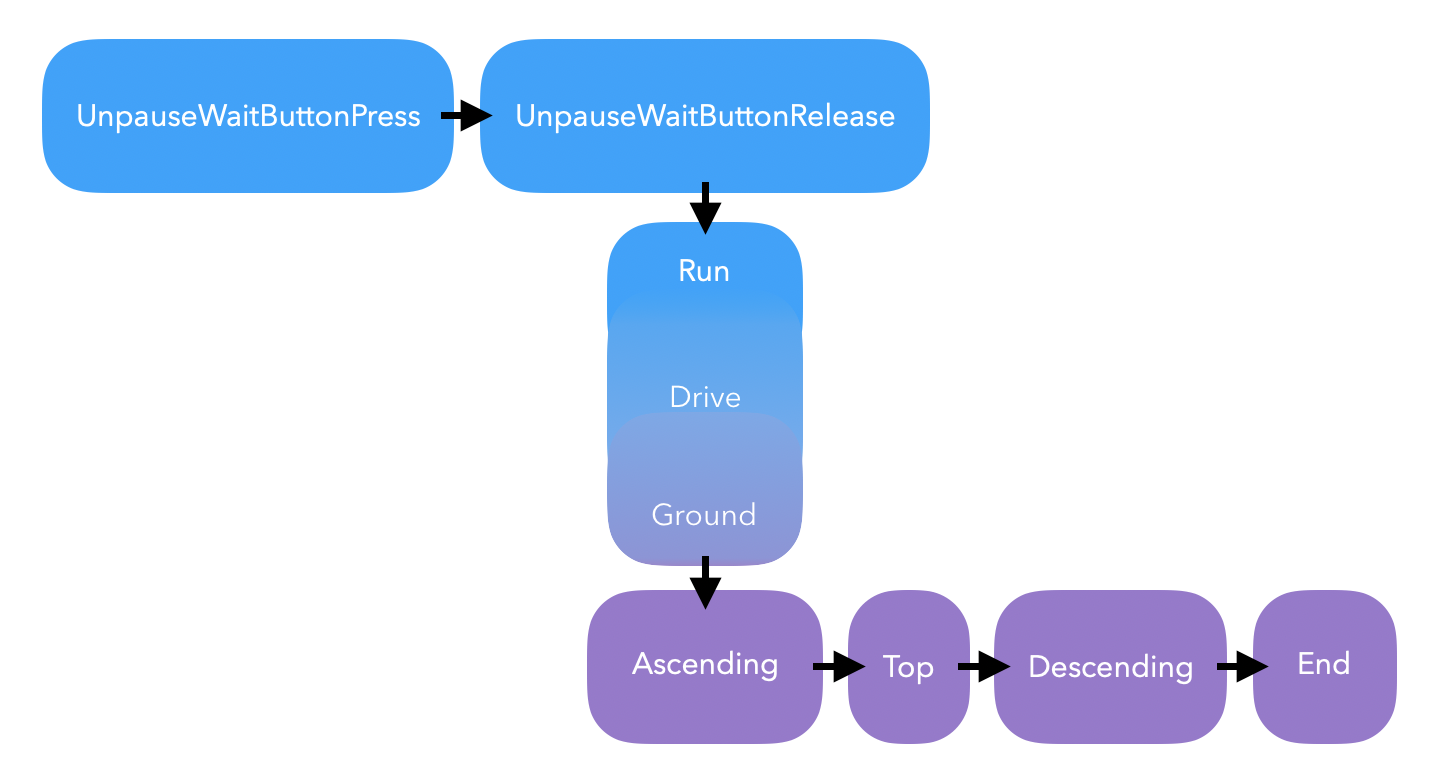
\includegraphics[width=11cm]{Images/EndTrace.png}
    \caption{A sample trace for the simplest path from \textit{UnpauseWaitButtonPress} to \textit{End}}
    \label{fig:endtrace}
\end{figure}
% do we need to consider LTL?

\subsection{Reliability} % do we need to talk about other theoretical stuff here?
In theory what could have been shown in the Kobuki final run was the transition from \textit{DriveAvoid} to \textit{Ascending} and this is a reachable path. By analysing the FSM, eventually (when incline conditions are met) the \textit{End} state is also reachable. However, physically it is not possible because the Kobuki would have no way of getting itself to the uphill ramp after losing ground orientation. This was an 'anticlockwise thinking' situation that was not considered when testing the FSM algorithms. If \textit{Run/Drive} was $T$ a target region, it would not be reachable from non-initial nodes in the hill climb hierarchy. To improve reliability, a transition back to the run/drive hierarchy would be necessary if incline detection becomes false. A time threshold must also be present to allow differentiation of the \textit{Top} state, where incline is also not true. More testing of the obstacle sensors over more extreme distances or obstacle situations would have encouraged robustness improvements. Having fine tuned actuation from sensors would mean the system is more reliable.